\documentclass[11pt,a4paper]{article}
\usepackage[T1]{fontenc}
\usepackage[utf8]{inputenc}
\usepackage{lmodern,microtype}
\usepackage{amsmath,amssymb,amsthm,mathtools,bm}
\usepackage{booktabs,array,tabularx,longtable}
\usepackage{graphicx,float,caption}
\usepackage{xcolor}
\usepackage[margin=20mm]{geometry}
\usepackage{enumitem}
\usepackage{fancyhdr}
\usepackage[hidelinks]{hyperref}
\hypersetup{
  pdftitle={FIN ST58--ST69: Interval Closure, Projective Sources, and the Thermodynamic Bridge},
  pdfauthor={Krzysztof Żuchowski},
  pdfsubject={Analytical and computational execution of FIN programs ST58--ST69},
  pdfkeywords={FIN, interval proof, spectral operator, projective state, chirality, thermodynamics, refinement, symmetry breaking}
}
\setlength{\parindent}{0pt}
\setlength{\parskip}{0.50em}
\setlength{\emergencystretch}{2em}
\setlength{\headheight}{14pt}
\setlist[itemize]{leftmargin=1.55em,itemsep=0.16em,topsep=0.2em}
\setlist[enumerate]{leftmargin=1.75em,itemsep=0.16em,topsep=0.2em}
\pagestyle{fancy}
\fancyhf{}
\lhead{FIN ST58--ST69}
\rhead{Release 10.59}
\cfoot{\thepage}
\newtheorem{theorem}{Theorem}[section]
\newtheorem{proposition}[theorem]{Proposition}
\newtheorem{corollary}[theorem]{Corollary}
\newcommand{\proven}{\textcolor{green!40!black}{\textbf{[PROVEN]}}}
\newcommand{\strong}{\textcolor{blue!70!black}{\textbf{[STRONG EVIDENCE]}}}
\newcommand{\conditional}{\textcolor{black!60}{\textbf{[CONDITIONAL]}}}
\newcommand{\constructed}{\textcolor{violet!70!black}{\textbf{[CONSTRUCTED]}}}
\newcommand{\failed}{\textcolor{red!72!black}{\textbf{[REFUTED IN CLASS]}}}
\newcommand{\statusboundary}{\textcolor{orange!80!black}{\textbf{[BOUNDARY]}}}
\newcommand{\resultbox}[1]{\begin{center}\fcolorbox{blue!60!black}{blue!4}{\parbox{0.92\textwidth}{#1}}\end{center}}

\begin{document}

\pagenumbering{gobble}
\begin{titlepage}
\centering
\vspace*{1.25cm}
{\LARGE\bfseries FIN ST58--ST69\par}
\vspace{0.35cm}
{\Large Interval Closure, Projective Sources, and the Thermodynamic Bridge\par}
\vspace{0.40cm}
{\large Full strict-to-memory certification, gain and spin-source obstructions, refinement falsification, CP intertwiners, chirality, and conditional thermodynamics\par}
\vspace{1.05cm}
{\Large Krzysztof Żuchowski\par}
\vspace{0.24cm}
{\large Independent Researcher --- Fractal Information Theory Project\par}
{\large ORCID: 0009-0002-0909-3613\par}
\vspace{0.85cm}
{\large FIN Release 10.59 --- Version 1.0.0\par}
{\large August 11, 2026\par}
\vfill
\begin{minipage}{0.89\textwidth}
\textbf{Scope.} This report executes ST58--ST69. It closes the outstanding arithmetic chain behind the FIN memory collision, attempts to source positive feedback and the projective selector state, tests a heat-signature refinement principle, strengthens the two-carrier protocol, derives the minimal conditional thermodynamic identity, and separates projective holonomy from chirality.\par
\textbf{Method.} Exact circulant and Fourier reductions, directed interval arithmetic, outward Krawczyk inclusions, finite-dimensional operator theory, Sturm root counts, information bounds, synthetic continuation, explicit countermodels, and twenty live tests.\par
\textbf{Epistemic rule.} Arithmetic closure does not imply physical closure. A constructed state or potential remains conditional until its source is derived. A failed search is not a nonexistence theorem.\par
\textbf{Repository snapshot.} Git commit \texttt{ac8d649f4f262abd010abe4546a51ae893ce5926}; the working tree contained additional local research artifacts recorded by the release manifest.\par
\textbf{Repository.} \url{https://github.com/hyconiek/Fractal-Nadsoliton-Theory}\par
\textbf{License.} CC BY 4.0.
\end{minipage}
\end{titlepage}
\pagenumbering{arabic}

\begin{abstract}
This report closes twelve local programs. ST58 is the principal proof-completion result. The strict operator, the even/odd hidden blocks, and the Stieltjes memory functions are circulant, so their projectors, residues, resolvents, and higher response operators reduce exactly to scalar Fourier intervals. An outward nonlinear Krawczyk inclusion certifies the localized stationary state, two outward linear inclusions certify the inverse quadratic forms, and interval evaluation isolates the collision speed in
\[
1.278014751813487\le s_*\le1.2780147518274094.
\]
The width is $1.40\times10^{-11}$. This closes the earlier upstream arithmetic gap under the declared exact circulant reduction. It is not a global Krein theorem or a proof-assistant replay.

ST59 proves a broad sign-flip obstruction: every adaptive-functional source class closed under $\Phi\mapsto-\Phi$ contains opposite linearized gains with identical stationarity and stabilizer data. The static strict core therefore cannot determine positive feedback. ST60 proves that every real two-dimensional strict spectral eigenspace is an integer Fourier doublet and has trivial Pancharatnam holonomy whenever the neighbor overlap is defined. The ST49 half-angle state requires projective/spin data absent from the scalar strict bundle.

ST61 refutes the proposed full heat-signature refinement source. Its first derivative forces the ST47 value $q=0$, but the directed interval for the normalized second-moment mismatch at $q=0$ is
\[
[-6.1281498283,-6.1281497880]\times10^{-5},
\]
which excludes zero. No declared dyadic lift preserves the complete normalized heat signature. ST62 bounds the frozen synthetic receiver's necessary and sufficient shots per preparation by 2 and 5, respectively; the prior 1,200-shot choice is deliberately far above this idealized bound.

ST63 classifies a completely positive operational intertwiner. Spectral pinching is CPTP, retains the 22-dimensional equal-eigenvalue block algebra, and intertwines unitary evolution with $A$-dephasing there, but is noninvertible. No invertible CP cross-channel equivalence exists. ST64 derives the exact conditional identity
\[
D(\rho\Vert\rho_\beta)=\frac{\widetilde\beta}{E_*}\bigl(F(\rho)-F(\rho_\beta)\bigr)
=\frac{\Delta S-Q/T}{k_B}.
\]
It also proves the remaining scale obstruction: $(E_*,T)\mapsto(cE_*,cT)$ leaves every dimensionless state and FIN record unchanged.

ST65 finds that the localized anti-continuum branch loses regular numerical continuation near coupling $0.0165$ and finds no localized root at strict coupling in 240 starts; this remains evidence, not nonexistence. ST66 supplies and completely classifies a smooth coercive polynomial $C_{12}$-equivariant selection model with twelve stable branches, but all gain and anisotropy coefficients are inserted. ST67 constructs a gauge-invariant Bargmann chirality that changes sign under reflection while both orientations retain $\pi$ holonomy, proving that flux and chirality are independent data. ST68 exports a calibration and custody validator. ST69 retains all nine physical source groups. Thus the arithmetic frontier advances, while selector, gain, scale, carrier, and physical-source frontiers remain open.
\end{abstract}

\textbf{Status vocabulary.} \proven{} denotes an analytic, exact finite, or outward interval result in the declared model. \strong{} denotes robust numerical evidence without global proof. \conditional{} denotes a theorem after explicit additional premises. \constructed{} denotes a complete mathematical object or protocol whose source is not derived. \failed{} means a proposed implication is destroyed in its declared class. \statusboundary{} records the precise non-implication.

\tableofcontents
\newpage

\section{Strict object, discipline, and questions}

The strict finite working operator remains
\begin{equation}
W_{xx}=0,\qquad
W_{xy}=\frac{\cos(0.18575d(x,y)+0.16250)}{1+d(x,y)^{1.8}}\quad(x\ne y),
\qquad A=sI-W,
\label{eq:strict}
\end{equation}
on $C_{12}$, with $s=1.6603072787660986$ to the displayed precision. Its positive weights imply
\[
\langle f,Af\rangle=\frac12\sum_{x,y}W_{xy}|f_x-f_y|^2\ge0.
\]
The zero diagonal is explicit. Inserting the scalar profile at $d=0$ would change the matrix and its row sum.

The legacy ontological kernel remains an intermediate bridge object, not a silent substitute for~\eqref{eq:strict}. This batch neither completes the legacy-to-strict bridge nor transfers the legacy claims for electroweak, electromagnetic, or hierarchy quantities.

The research questions are:
\begin{enumerate}
\item Can the complete collision chain be certified without freezing upstream floating coefficients?
\item Can positive gain or the projective texture be derived from the strict scalar operator?
\item Can an intrinsic heat or compression signature select a unique refinement?
\item Which operational equivalences survive complete positivity and finite counts?
\item What is the smallest honest bridge from information entropy to thermodynamics?
\item Can localization, smooth symmetry breaking, and chirality be obtained without promoting constructed laws to strict physics?
\end{enumerate}

\resultbox{\textbf{Principal conclusion.} ST58 removes a genuine mathematical uncertainty: the declared collision is now interval-certified from the exact-decimal strict kernel through the memory reduction. The physical obstruction is unchanged. The same batch proves that the static strict core does not source gain sign or the required projective half-angle texture.}

\section{Outcome matrix}

\small
\begin{longtable}{@{}p{0.055\textwidth}p{0.30\textwidth}p{0.23\textwidth}p{0.34\textwidth}@{}}
\toprule
ID & Object & Outcome & Exact boundary\\
\midrule
\endfirsthead
\toprule
ID & Object & Outcome & Exact boundary\\
\midrule
\endhead
ST58 & Full strict-to-memory collision certificate & \proven{} & Not proof-assistant or global Krein theorem\\
ST59 & Adaptive gain-source audit & \proven{} no-go & Time-oriented classes remain open\\
ST60 & Strict projective-source audit & \proven{} obstruction & Added spin/projective structure remains possible\\
ST61 & Heat-signature refinement & \failed{} & Other nonstationary fractal codes remain open\\
ST62 & Finite-count information bounds & \proven{} conditional & Frozen synthetic probability tables\\
ST63 & CP channel intertwiner & \proven{} & Uses $A$-dephasing, not vertex heat directly\\
ST64 & Information-to-thermodynamics bridge & \conditional{} & $E_*,k_B$, bath, and instrument added\\
ST65 & Localized excited-state search & \strong{} negative search & No global nonexistence theorem\\
ST66 & Smooth $C_{12}$ bifurcation & \proven{} constructed & Gain and branch event inserted\\
ST67 & $\pi$ holonomy versus chirality & \proven{} conditional & Chiral $\mathbb{CP}^1$ texture inserted\\
ST68 & Calibration/custody validator & \constructed{} & Cannot create independence or external records\\
ST69 & Updated axiom graph & \proven{} relative no-reduction & Nine source groups retained\\
\bottomrule
\end{longtable}
\normalsize

\section{ST58 --- Full directed-interval collision certificate}

\subsection{Exact Fourier reduction}

The key observation is structural. Because $A$ is radial on $C_{12}$, it is a real symmetric circulant. Splitting the vertices into even and odd sites produces $6\times6$ circulant blocks
\[
B=A_{\rm even,odd},\qquad C=A_{\rm odd,odd}+\frac{3}{20}I.
\]
Both are exactly diagonalized by the six-point discrete Fourier transform. If $p_j$ are the distinct eigenvalues of $C$ and $P_j$ their spectral projectors, the grouped residues are
\[
r_j=\frac1{6}\operatorname{tr}(BP_jB^T).
\]
In Fourier coordinates these become scalar squared moduli with multiplicities $1,2,2$. The fourth hidden mode has exactly zero residue because its alternating $B$ eigenvalue cancels:
\[
-w_1+w_3-w_5+w_5-w_3+w_1=0.
\]
No floating eigenvector grouping is required.

The memory and its two response derivatives are spectral functions of $A$:
\begin{align*}
M&=\sigma(0)I-\sum_jr_j(A+p_jI)^{-1},\\
T&=\sum_jr_j(A+p_jI)^{-2},\\
S&=\sum_jr_j(A+p_jI)^{-3}.
\end{align*}
Every eigenvalue is evaluated from the exact decimals
\[
\omega=\frac{743}{4000},\quad \phi=\frac{13}{80},\quad
\eta=\frac95,\quad \beta=1,
\]
using 80-digit directed intervals. Inverse Fourier reconstruction then provides outward entry intervals for $A+M$, $T$, and $S$.

\subsection{Nonlinear and linear inclusions}

The stationary equation is
\[
(A+M)u+u-u^{\circ3}=0.
\]
An interval Krawczyk operator around the localized center has maximum state radius $10^{-13}$, maximum image radius $2.18\times10^{-14}$, and minimum strict inclusion margin $7.82\times10^{-14}$. The infinity-norm defect bound is $2.56\times10^{-13}$. A separate $2\times10^{-14}$ per-component arithmetic payment covers the remaining fixed binary64 preconditioner operations.

Two linear Krawczyk inclusions then enclose
\[
L_+^{-1}u,\qquad L_+^{-1}Tu,qquad
L_+=A+M+I-3\operatorname{diag}(u^2).
\]
The spectral radii of their nonnegative comparison matrices are about $2.34\times10^{-13}$; the strict inclusion margins are $2.14\times10^{-14}$ and $2.05\times10^{-14}$.

The Jordan coefficients satisfy
\[
\kappa(s)=-\left(c_0+\frac{2c_1}{s}+\frac{c_2+c_3}{s^2}\right),
\]
where
\[
c_0=\langle u,L_+^{-1}u\rangle,quad
c_1=\langle u,L_+^{-1}Tu\rangle,quad
c_2=\langle Tu,L_+^{-1}Tu\rangle,quad
c_3=\langle u,Su\rangle.
\]
The outward coefficient intervals are
\begin{align*}
0.2671565201184344&\le c_2+c_3\le0.2671565201188138,\\
0.1122179451840949&\le2c_1\le0.1122179451854801,\\
-0.2513728361103568&\le c_0\le-0.2513728361084486.
\end{align*}

\begin{theorem}[Full declared-chain interval certificate]
Under the exact circulant/Fourier reduction and exact-decimal strict input, the localized stationary branch contains a unique state in the certified box and the positive collision speed lies in
\[
1.278014751813487\le s_*\le1.2780147518274094.
\]
\end{theorem}

\begin{figure}[H]
\centering
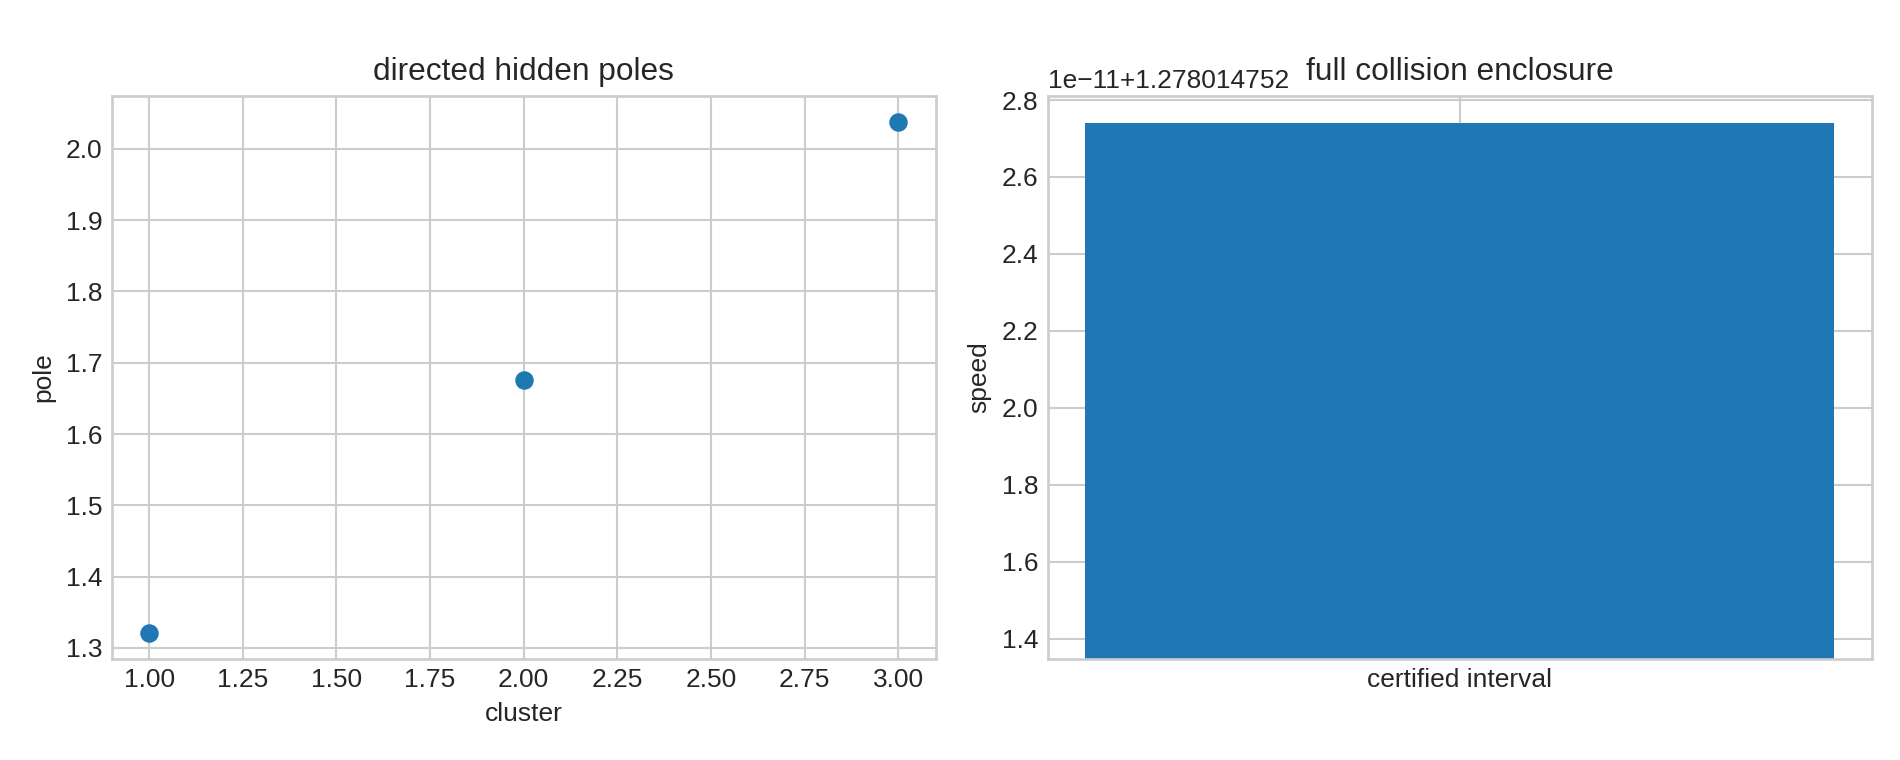
\includegraphics[width=0.90\textwidth]{FIN_ST58_ST69_Figures/st58_full_interval.png}
\caption{Directed hidden poles and the final collision enclosure. The interval height is displayed on the absolute speed axis.}
\end{figure}

\statusboundary{} The certificate proves the stated finite arithmetic chain. It does not prove global spectral stability, uniqueness of every nonlinear branch, a continuum limit, a physical clock, or a Krein theorem beyond the declared reduction. An independent interval library or proof assistant is recommended as ST70.

\section{ST59 --- Why the static core cannot select positive gain}

Let $P_-$ and $P_+$ denote reflection-odd and reflection-even perturbation sectors. Suppose an admissible response-functional class is closed under multiplication by $-1$. For any $\Phi$ in the class, $-\Phi$ has the same stationarity condition at $A$ and the same stabilizer invariance, but its Hessian has the opposite sign. Gradient flow therefore reverses its linearized gain.

The elementary witness pair is
\[
\Phi_\pm(A+H)=\pm\frac12\left(\|P_-H\|_F^2+\|P_+H\|_F^2\right).
\]
Both are stationary at $A$ and reflection invariant. Their odd gains under negative gradient flow are $\mp1$.

\begin{theorem}[Sign-closed source obstruction]
No source class closed under $\Phi\mapsto-\Phi$ can derive the sign of adaptive gain from stationarity and stabilizer data alone. A positive-gain theorem requires an additional order, time orientation, entropy-production direction, Lyapunov convention, or equivalent premise.
\end{theorem}

\begin{figure}[H]
\centering
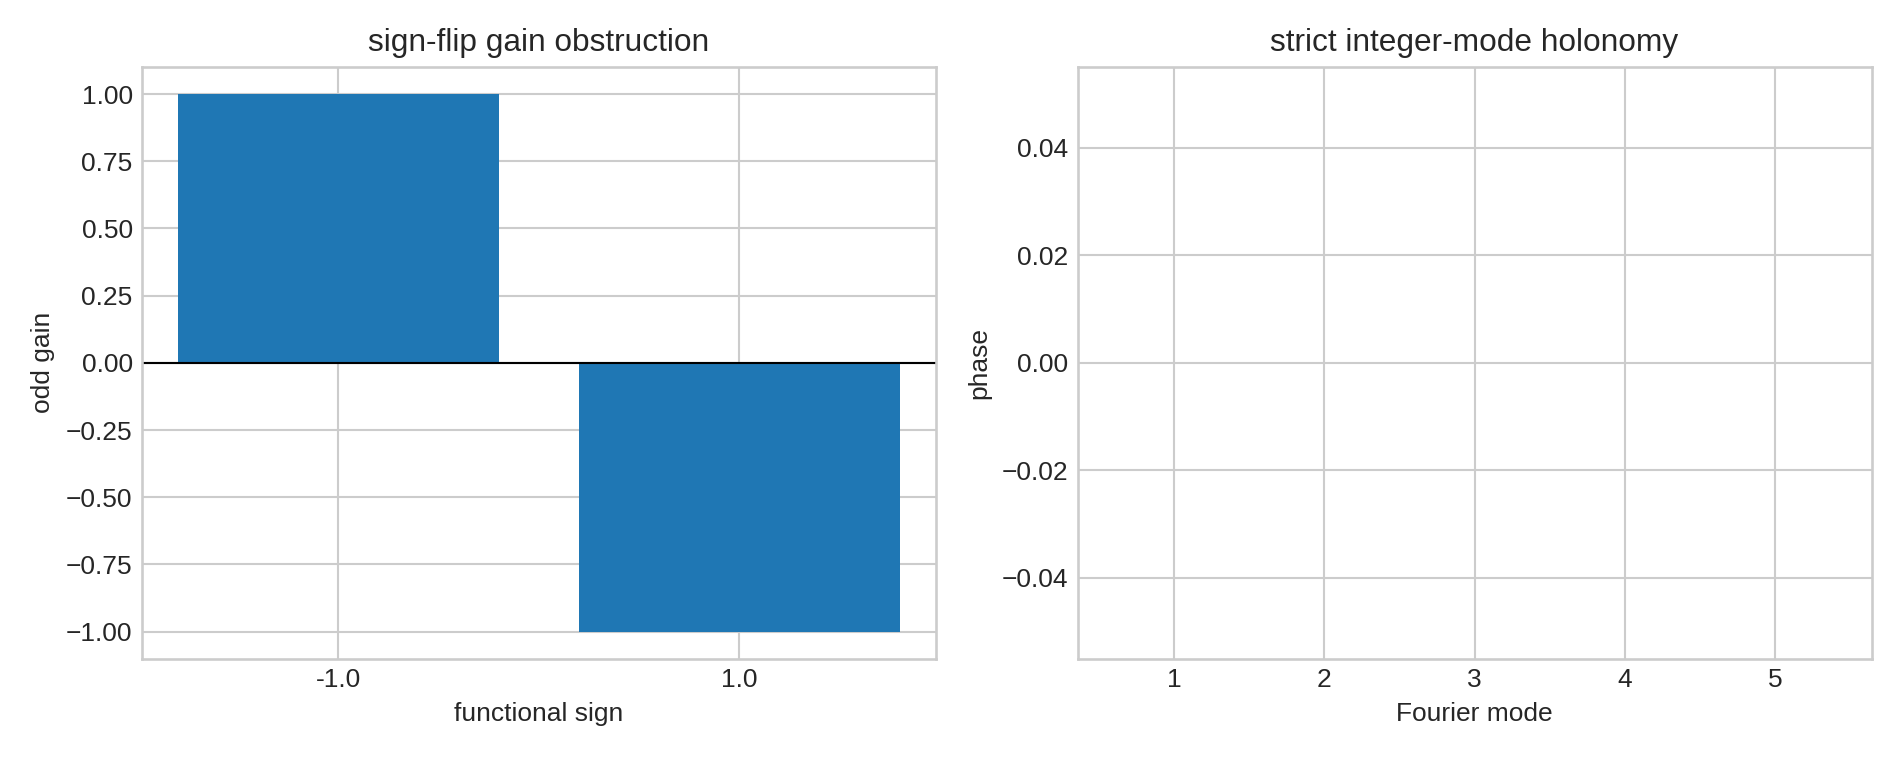
\includegraphics[width=0.96\textwidth]{FIN_ST58_ST69_Figures/st59_gain_st60_projective_source.png}
\caption{Left: identical static source data permit opposite gains. Right: all defined integer Fourier ray embeddings have zero holonomy phase.}
\end{figure}

\statusboundary{} The result strengthens ST48 but does not prove that gain can never be sourced. It identifies what a successful source must add: a mathematically oriented response principle not invariant under global functional sign reversal.

\section{ST60 --- The scalar strict bundle does not contain the half-angle texture}

Every real two-dimensional eigenspace of a scalar $C_{12}$ circulant is an integer Fourier doublet
\[
r_x^{(k)}=\left(\cos\frac{2\pi kx}{12},\sin\frac{2\pi kx}{12}\right),
\qquad k=1,\ldots,5.
\]
Its neighbor overlap is constant:
\[
\langle r_x^{(k)},r_{x+1}^{(k)}\rangle=\cos\frac{2\pi k}{12}.
\]
Whenever this is nonzero, the twelve-link Pancharatnam product is
\[
\operatorname{sgn}\left(\cos\frac{2\pi k}{12}\right)^{12}=+1.
\]
For $k=3$ the neighbor rays are orthogonal and the link phase is undefined. Thus no defined integer doublet has the $-1$ holonomy of ST49.

\begin{theorem}[Half-integer spectral-source obstruction]
The scalar strict spectral bundle does not generate the ST49 projective half-angle texture. Achieving holonomy $-1$ requires a half-integer lift, spin structure, central extension, antiperiodic boundary condition, or another explicitly added projective object.
\end{theorem}

This is stronger than saying that no preferred axis was found. The representation type itself is missing from the scalar bundle. It also explains why adding more scalar functions of $A$ cannot solve this particular obstruction.

\statusboundary{} A projective extension remains mathematically admissible. The theorem says that it is new data and is not hidden in the existing integer Fourier eigenspaces. QW-2191 remains open.

\section{ST61 --- Full heat-signature refinement fails}

For a proposed refinement $A_{24}(q)$, exact normalized heat-trace stationarity would require
\[
\frac1{24}\operatorname{tr}e^{-tA_{24}(q)}
=\frac1{12}\operatorname{tr}e^{-tA_{12}}qquad\text{for all }t\ge0.
\]
Equality of the first derivative at $t=0$ gives the ST47 trace equation and forces $q=0$. Equality of the second derivative would then require
\[
\frac1{24}\operatorname{tr}A_{24}(0)^2
=\frac1{12}\operatorname{tr}A_{12}^2.
\]
Directed intervals from the exact-decimal strict weights instead give
\[
\frac1{24}\operatorname{tr}A_{24}(0)^2-
\frac1{12}\operatorname{tr}A_{12}^2
\in[-0.0000612814982830,-0.0000612814978798].
\]

\begin{theorem}[No heat-stationary declared lift]
No $q\ge0$ in the declared dyadic family preserves the complete normalized heat signature. The first moment forces $q=0$, while the second moment excludes it.
\end{theorem}

\begin{figure}[H]
\centering
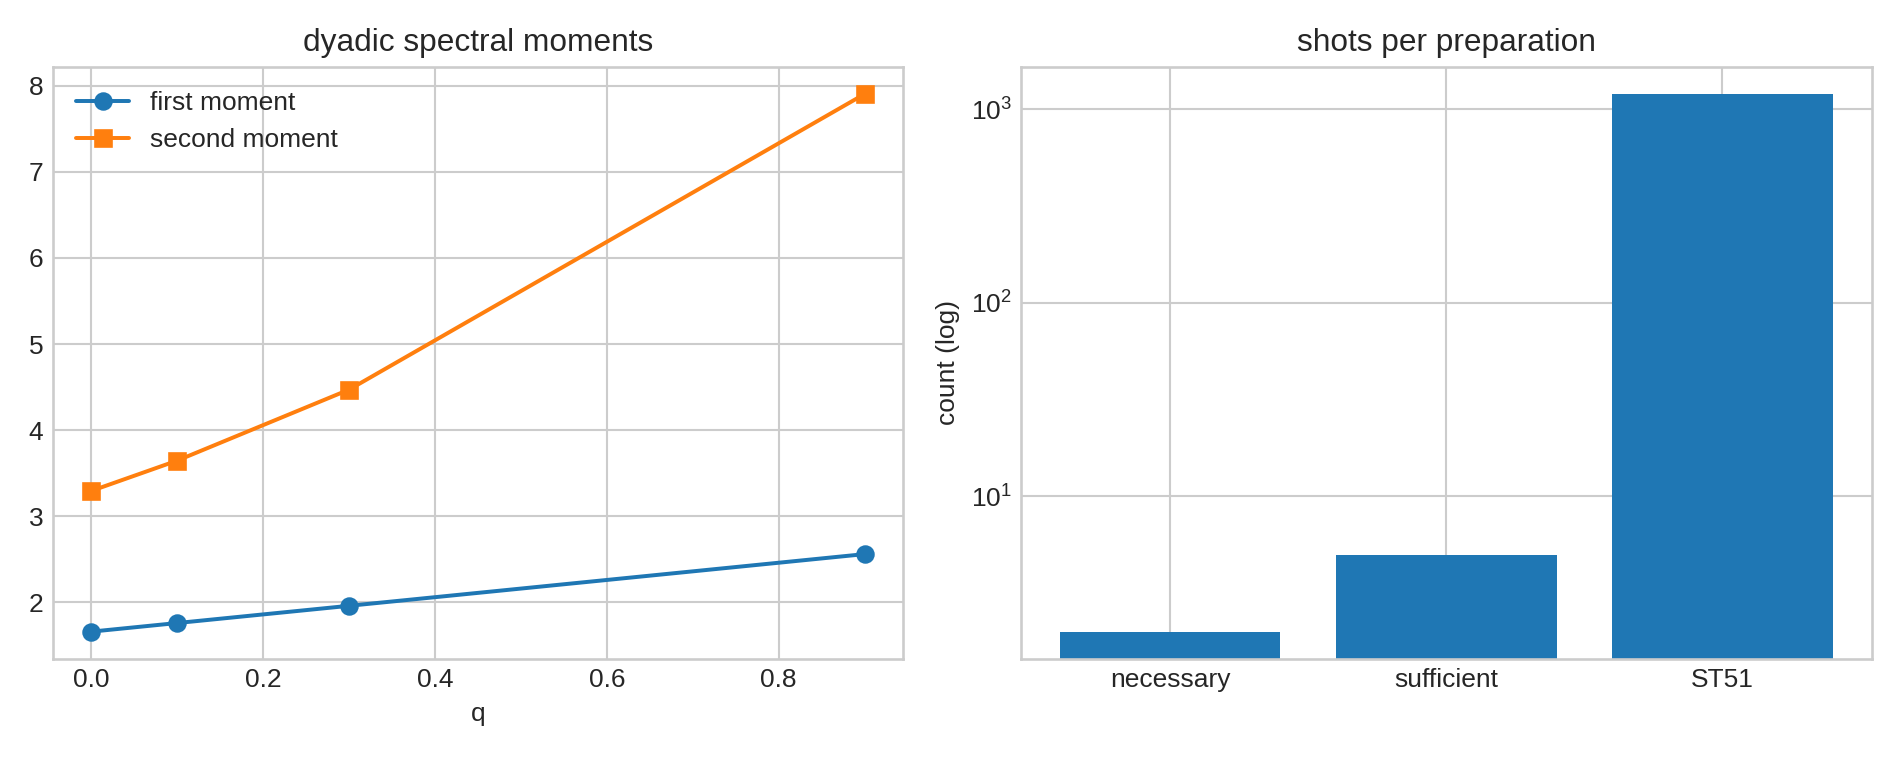
\includegraphics[width=0.96\textwidth]{FIN_ST58_ST69_Figures/st61_refinement_st62_counts.png}
\caption{Left: trace and second-moment densities along the lift family. Right: analytic necessary/sufficient synthetic count bounds compared with the ST51 budget.}
\end{figure}

\statusboundary{} This is a useful falsification, not a rejection of fractal compression. A nonstationary renormalization law or fine-data rate-distortion code may still exist. It must specify how information changes across levels rather than demand exact heat-signature identity.

\section{ST62 --- Finite-count information bounds}

Let $P_x$ and $Q_x$ be the frozen carrier-A and mismatched carrier-B outcome distributions for preparation $x$. With $n$ events per preparation, the total Kullback--Leibler divergences are
\[
n\sum_xD(P_x\Vert Q_x),\qquad n\sum_xD(Q_x\Vert P_x),
\]
with one-shot sums $4.14379$ and $5.04802$.

If both type-I and type-II errors are at most $\epsilon=0.01$, binary data processing gives the necessary bound
\[
n\ge2.
\]
The optimized Chernoff information is $C=0.95449136$ at $s=0.47258409$. Hence the optimal likelihood-ratio error sum obeys
\[
\alpha+\beta\le e^{-nC},
\]
and $n=5$ is sufficient for both errors to be at most $0.01$. Thus the mathematical bracket is
\[
2\le n_{\min}\le5
\]
for the frozen ideal probability tables. ST51 used $1,200$ events per preparation.

\statusboundary{} The surprisingly small bracket measures the deliberately large synthetic mismatch. It is not a recommended laboratory count. Dark counts, nuisance calibration, drift, loss, apparatus nonideality, and independent custody are absent.

\section{ST63 --- Completely positive intertwiners}

To place channel comparison in a genuine quantum-operational setting, define
\[
\mathcal U_t(\rho)=e^{-itA}\rho e^{itA},\qquad
\mathcal D_\tau(\rho)=e^{-\tau\operatorname{ad}_A^2}(\rho).
\]
On a matrix unit between eigenmodes $i,j$, their superoperator eigenvalues are
\[
e^{-it(\lambda_i-\lambda_j)},\qquad e^{-\tau(\lambda_i-\lambda_j)^2}.
\]
At $t=\tau=0.61$, equality requires $\lambda_i=\lambda_j$ because the second value has modulus below one for every nonzero gap while the first has modulus one.

The canonical surviving map is spectral pinching
\[
\Pi(\rho)=\sum_{\alpha=1}^{7}P_\alpha\rho P_\alpha.
\]
It is CPTP, its Choi matrix is positive to a numerical lower residual of $-1.4\times10^{-15}$, and its trace-preservation residual is $4.2\times10^{-15}$. The multiplicities
\[
(1,2,2,2,2,2,1)
\]
give output block-algebra dimension $22$.

\begin{theorem}[CP pinching and no invertible equivalence]
Spectral pinching intertwines the unitary and $A$-dephasing channels only after all cross-eigenspace coherences are destroyed. It is noninvertible, and no invertible completely positive cross-channel intertwiner exists at the declared parameters.
\end{theorem}

\begin{figure}[H]
\centering
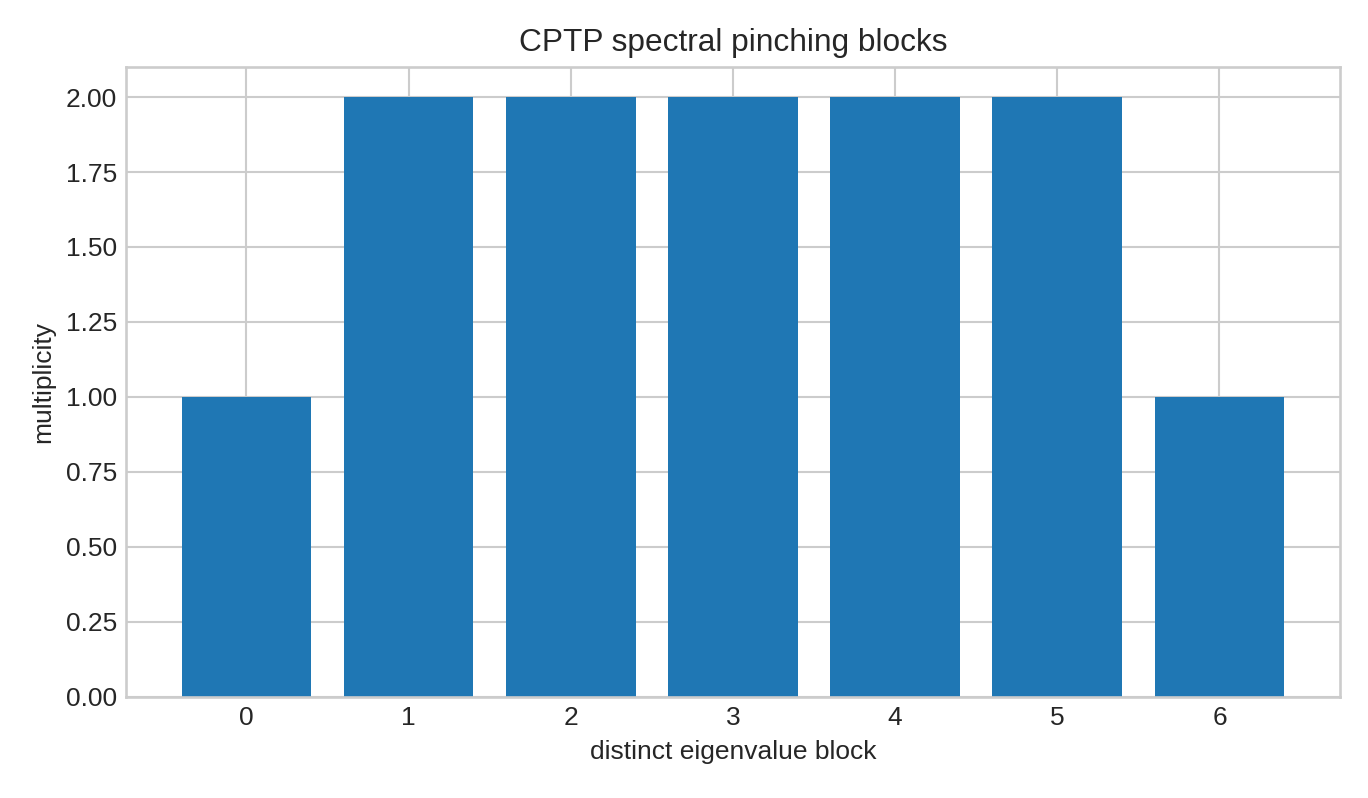
\includegraphics[width=0.76\textwidth]{FIN_ST58_ST69_Figures/st63_cp_pinching.png}
\caption{Seven spectral blocks retained by the CPTP pinching channel. Their squared multiplicities sum to 22.}
\end{figure}

\statusboundary{} The dephasing channel is a valid $A$-derived quantum channel. It is not the classical vertex Markov semigroup $e^{-\tau A}$ acting on probabilities. The result prevents those two meanings from being silently merged.

\section{ST64 --- The smallest honest thermodynamic bridge}

Add an energy unit $E_*>0$ and define
\[
H=E_*A,qquad
\rho_{\widetilde\beta}=\frac{e^{-\widetilde\beta A}}{\operatorname{tr}e^{-\widetilde\beta A}}.
\]
Add an entropy unit $k_B$ and set $S(\rho)=k_BS_{\rm vN}(\rho)$. The physical temperature compatible with the dimensionless Gibbs parameter is
\[
T=\frac{E_*}{k_B\widetilde\beta}.
\]
For a bath process taking $\rho$ to $\rho_{\widetilde\beta}$, with $Q=\operatorname{tr}H(\rho_{\widetilde\beta}-\rho)$,
\begin{align*}
D(\rho\Vert\rho_{\widetilde\beta})
&=\frac{\widetilde\beta}{E_*}\left[F(\rho)-F(\rho_{\widetilde\beta})\right],\\
\Delta S-\frac QT&=k_BD(\rho\Vert\rho_{\widetilde\beta})\ge0.
\end{align*}
The frozen numerical identity residuals are below $1.7\times10^{-15}$.

\begin{theorem}[Conditional thermodynamic bridge and scale obstruction]
The Gibbs/free-energy/entropy-production bridge is exact after adding $E_*$, $k_B$, a bath equilibrium state, and a thermalization process. These dimensional inputs are not recoverable from dimensionless FIN data because
\[
(E_*,T)\mapsto(cE_*,cT)
\]
leaves $\widetilde\beta$, the Gibbs state, and every dimensionless record invariant.
\end{theorem}

\begin{figure}[H]
\centering
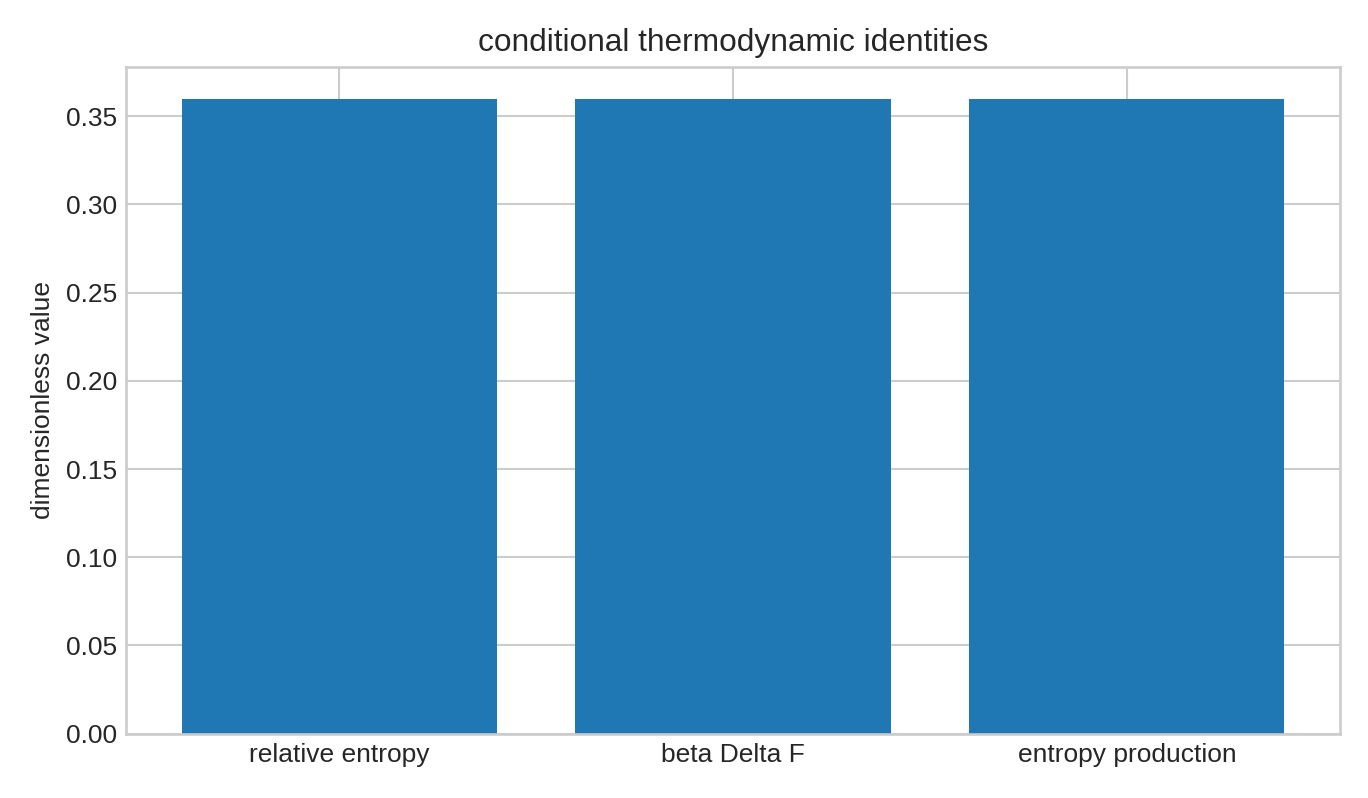
\includegraphics[width=0.76\textwidth]{FIN_ST58_ST69_Figures/st64_thermodynamic_bridge.png}
\caption{Three numerical evaluations of the same conditional relative-entropy identity.}
\end{figure}

\statusboundary{} This is the shortest bridge found in the current finite setting, but it is an axiom-augmented bridge. FIN does not strict-derive $E_*$, $k_B$, a bath, heat/work semantics, or temperature calibration.

\section{ST65 --- Localized excited-state search remains unresolved}

The constructed saturating energy has an exact uniform ground-state orbit. ST65 asks whether a localized excited critical point survives at full strict coupling. Starting from one high-amplitude site at the anti-continuum limit, ordinary parameter continuation retains a sharply localized branch only to $\kappa=0.0165$, where the last regular point has IPR $0.97978$. The next Newton step loses regular convergence, consistent with a nearby fold.

At full coupling $\kappa=1$, 240 deterministic random starts produce 166 converged stationary solutions and no solution with IPR above $0.10$.

\begin{figure}[H]
\centering
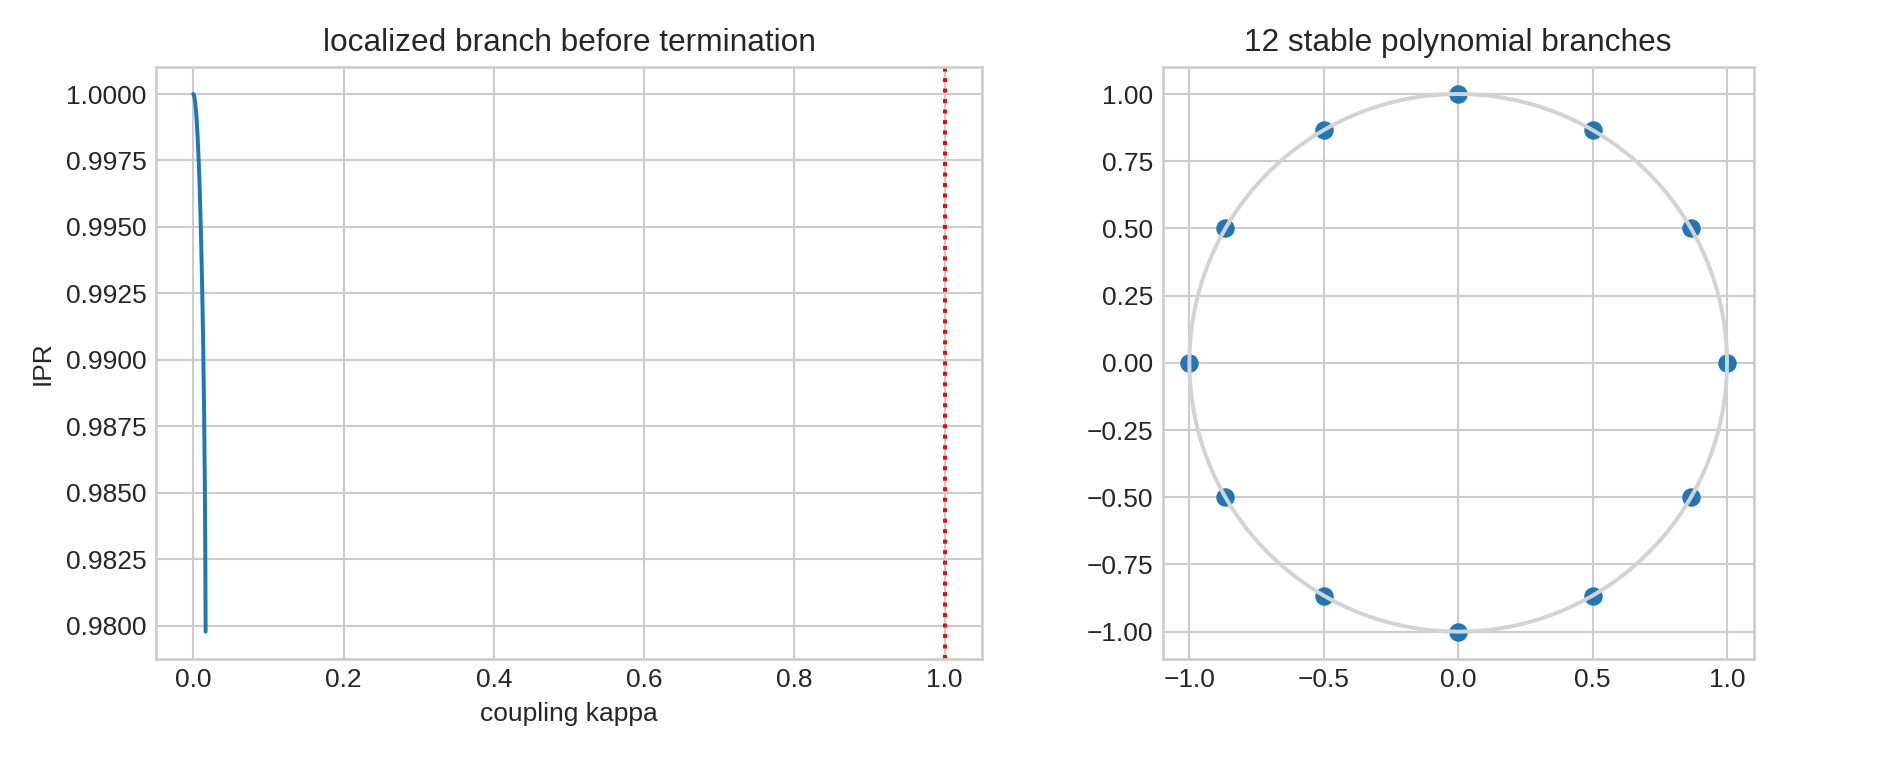
\includegraphics[width=0.96\textwidth]{FIN_ST58_ST69_Figures/st65_localization_st66_bifurcation.png}
\caption{Left: the regular localized continuation terminates far below strict coupling. Right: the twelve stable axes of the constructed polynomial selection model.}
\end{figure}

\strong{} The declared search supplies strong negative evidence for a connected localized branch reaching $\kappa=1$.

\statusboundary{} It does not prove global nonexistence. A fold can be traversed by pseudo-arclength, and disconnected branches may evade multistart root finding. ST77 must certify the fold or continue through it before any nonexistence claim.

\section{ST66 --- A smooth polynomial selection mechanism}

The earlier polar model was not smooth at the origin. ST66 replaces it by the coercive polynomial potential
\[
V(z)=-\frac\mu2|z|^2+\frac14|z|^4
-\frac\epsilon{12}\operatorname{Re}(z^{12})
+\frac\nu{14}|z|^{14},
\]
with
\[
\mu=\frac7{20},\qquad \epsilon=\nu=\frac1{100}.
\]
It is invariant under $z\mapsto e^{2\pi i/12}z$ and reflection $z\mapsto\bar z$.

Writing $y=|z|^2$, the stable angular classes satisfy
\[
-\frac7{20}+y-\frac1{100}y^5+\frac1{100}y^6=0.
\]
Sturm counting proves exactly one positive root. The opposite angular classes also have exactly one positive root. The $\cos(12\theta)=+1$ roots give twelve local minima with radial curvature $0.69976$ and angular curvature $2.2072\times10^{-4}$; the $\cos(12\theta)=-1$ roots give twelve angular saddles. The origin is unstable because $\mu>0$.

\begin{theorem}[Smooth finite branch classification]
The displayed polynomial flow provides a globally smooth, coercive, $C_{12}$-equivariant symmetry-breaking mechanism with exactly twelve stable nonzero branches and twelve angular saddles.
\end{theorem}

\statusboundary{} This proves mathematical sufficiency, not strict origin. Gain, saturation, anisotropy, coupling to the strict doublet, and the realized history are inserted.

\section{ST67 --- Holonomy and chirality are different data}

The real half-angle state has $\pi$ holonomy but no gauge-invariant local complex chirality. To separate the two roles, ST67 constructs normalized $\mathbb{C}P^1$ rays
\[
\psi_x=\begin{pmatrix}
\sqrt{1-t}\\ \sqrt t\,e^{2\pi i(2x)/12}
\end{pmatrix},\qquad t=2-\sqrt3.
\]
Each forward link has phase $\pi/12$, so the twelve-link Pancharatnam product is $-1$. Reflection inverts the path but retains the same $-1$ holonomy.

Define the gauge-invariant Bargmann chirality
\[
\chi_B=\sum_x\operatorname{Im}\left(
\langle\psi_x,\psi_{x+1}\rangle
\langle\psi_{x+1},\psi_{x+2}\rangle
\langle\psi_{x+2},\psi_x\rangle\right).
\]
The forward and reflected textures give
\[
\chi_B=+0.9460598986,qquad \chi_B=-0.9460598986,
\]
while both retain $\mathcal H=-1$.

\begin{theorem}[$\pi$ flux does not encode chirality]
Projective holonomy and orientation are independent. Reflection fixes the $\pi$ holonomy class but reverses the Bargmann chirality.
\end{theorem}

\begin{figure}[H]
\centering
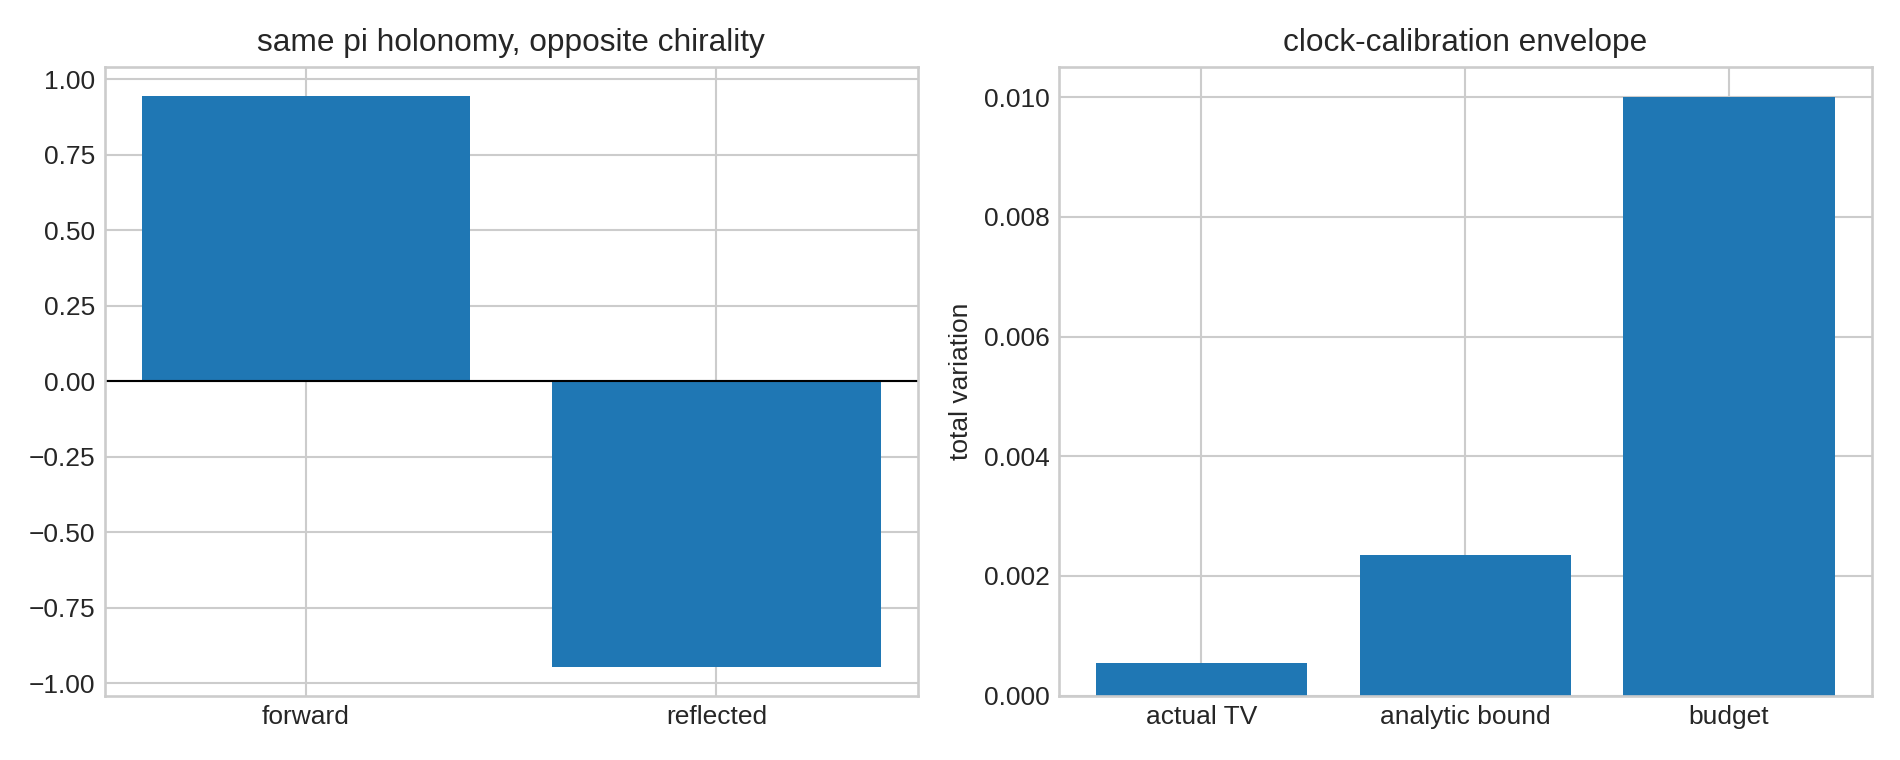
\includegraphics[width=0.96\textwidth]{FIN_ST58_ST69_Figures/st67_chirality_st68_validator.png}
\caption{Left: equal $\pi$ holonomy with opposite projective chirality. Right: actual clock mismatch, analytic envelope, and frozen TV budget.}
\end{figure}

\statusboundary{} The chiral texture is inserted and not strict-sourced. The theorem prevents the admissibility of $\pi$ holonomy from being misreported as an orientation selector.

\section{ST68 --- Calibration and custody validation}

For a unitary evolution with generator norm $\|A\|=2.34218204$, a clock error $|\delta t|\le10^{-3}$ gives the state/measurement bound
\[
\operatorname{TV}\le\|A\||\delta t|\le0.00234219.
\]
The actual worst endpoint TV for the frozen vertex experiment is $0.00054915$, below both this analytic bound and the declared budget $0.01$.

The executable validator requires seven event fields, four pairwise distinct role identifiers, a hash frozen before unblinding, a frozen hold-out, one pipeline run, and no post-failure refit. It accepts the complete synthetic example and rejects both a duplicated provider/registrar identity and a missing external-record flag. Its specification hash is
\[
\texttt{72ab3694cd530a703b3e0d17a94a6c2646523ba70700490b73655839cd90162b}.
\]

\statusboundary{} A validator can reject an invalid packet. It cannot cause the named humans or institutions to be independent, certify an apparatus, or create raw external events. Those are physical and governance facts outside local code.

\section{ST69 --- Updated axiom graph}

The nine source groups remain:
\begin{center}
\small
\begin{tabularx}{0.96\textwidth}{@{}l l X@{}}
\toprule
Group & Status & ST58--ST68 reason\\
\midrule
A0 strict finite operator & retained & ST58 certifies consequences, not the source of $A$\\
A1 state-selection event & retained & ST60 obstructs; ST66/ST67 insert states/branches\\
A2 refinement law & retained & ST61 refutes full heat stationarity\\
A3 dimensional calibration & retained & ST64 proves the positive scale orbit\\
A4 operational process & constructible & ST63/ST68 refine its form\\
A5 external custody/data & retained & ST68 cannot generate independence/events\\
A6 nonlinear response/gain & retained & ST59 proves sign nonidentifiability\\
A7 connection/projective sector & retained & ST60 obstructs; ST67 inserts $\mathbb{C}P^1$ data\\
A8 temporal memory realization & retained & ST58 certifies one static reduction, not temporal uniqueness\\
\bottomrule
\end{tabularx}
\end{center}

Conditional packages do compress bookkeeping. A chiral projective state packages A1 and A7; a smooth selected order parameter packages A1 and A6; the thermal conversion package supplies A3 plus bath semantics; the validator packages A4 plus a record schema. None is strict-derived.

\begin{theorem}[No strict source-group reduction]
ST58 closes an arithmetic obligation, while ST59--ST68 either prove an obstruction or construct an explicitly conditional object. All nine physical-completion source groups remain necessary relative to the declared targets and construction classes.
\end{theorem}

\section{Falsification ledger and current interpretation}

This batch makes the research map substantially sharper:
\begin{itemize}
\item \textbf{Arithmetic uncertainty removed.} The collision is no longer only a strong floating result in the declared finite model.
\item \textbf{Gain-source class closed.} Static stationarity and symmetry cannot select gain in any sign-closed functional class.
\item \textbf{Scalar-projector route closed.} Integer strict Fourier doublets cannot generate the half-angle $-1$ texture.
\item \textbf{Heat-fixed refinement closed.} First and second spectral moments are incompatible with complete heat-signature stationarity.
\item \textbf{Channel equivalence narrowed.} A CPTP pinching quotient exists, but an invertible operational equivalence does not.
\item \textbf{Thermodynamic bridge isolated.} The correct relative-entropy identities emerge after $E_*$, $k_B$, bath, and process data are supplied; the positive scale orbit proves why these are not internally identifiable.
\item \textbf{Localization remains open.} The numerical branch fails early, but a global theorem was not obtained.
\item \textbf{Symmetry breaking constructed, not sourced.} A smooth polynomial mechanism exists, locating exactly which coefficients require explanation.
\item \textbf{Flux separated from orientation.} $\pi$ holonomy cannot be used as a hidden chirality selector.
\end{itemize}

The deepest mathematical interpretation surviving this batch is an \emph{interval-certifiable finite spectral-information core with nonunique physical completion}. Its operator consequences can be proved increasingly sharply. The missing physics resides not in numerical precision but in typed source objects: time orientation/response, projective sector, refinement law, dimensions, operational realization, and external record.

This is consistent with, but does not prove, the FIN ontology of the nadsoliton as primordial fractal information in a solitonic state. No independent informational layer is introduced. The internal order remains nadsoliton $\rightarrow$ light $\rightarrow$ matter $\rightarrow$ emergent observer.

\section{Recommended next programs ST70--ST81}

\small
\begin{longtable}{@{}p{0.08\textwidth}p{0.10\textwidth}p{0.74\textwidth}@{}}
\toprule
Program & Priority & Research test\\
\midrule
\endfirsthead
\toprule
Program & Priority & Research test\\
\midrule
\endhead
ST70 & 1 & Independently replay ST58 with another interval library or proof assistant.\\
ST71 & 2 & Classify monotone or time-oriented adaptive response classes that evade the ST59 sign-flip obstruction.\\
ST72 & 3 & Derive or obstruct a spin structure or central extension from one genuinely new strict-sourced object.\\
ST73 & 4 & Construct a nonstationary fine-data fractal rate-distortion/RG law and test uniqueness of refinement.\\
ST74 & 5 & Derive a minimax finite-count design including calibration nuisance, loss, and dark-count channels.\\
ST75 & 6 & Classify all CPTP intertwiners through Choi-semidefinite constraints, beyond spectral Schur maps.\\
ST76 & 7 & Prove a resource-theoretic minimality theorem for the $E_*,k_B$, bath conversion package.\\
ST77 & 8 & Pseudo-arclength continue the ST65 fold and interval-certify termination or a return branch.\\
ST78 & 9 & Couple the ST66 order parameter to the strict first Fourier doublet and audit backreaction without claiming a source.\\
ST79 & 10 & Search for a strict-sourced orientation-odd Bargmann observable or prove its stabilizer obstruction.\\
ST80 & 11 & Export a laboratory-neutral event validator with signed custody attestations and frozen nuisance bounds.\\
ST81 & 12 & Update the W0+CA+SA architecture and nine-source graph after ST70--ST80.\\
\bottomrule
\end{longtable}
\normalsize

The highest-value conceptual lane is now ST71--ST73: the static routes are closed in broad classes, so progress requires one new typed source---time orientation, spin/projective structure, or a nonstationary fractal code. ST70 remains valuable as independent proof reproducibility rather than new physics.

\section{Reproducibility}

The release packet contains:
\begin{itemize}
\item \texttt{fin\_st58\_st69\_research.py} --- deterministic analysis and seven figures;
\item \texttt{test\_fin\_st58\_st69.py} --- twenty live acceptance tests;
\item the complete JSON/CSV ledger;
\item the ST58 interval certificate, ST62 count-bound packet, and ST68 executable validator;
\item a frozen input inventory and release SHA-256 manifest.
\end{itemize}

The seed is 20260814 and dependency versions are serialized. The complete local replay is
\[
\texttt{MPLCONFIGDIR=/tmp/fin-st58-mpl python3 fin\_st58\_st69\_research.py}
\]
followed by
\[
\texttt{MPLCONFIGDIR=/tmp/fin-st58-mpl python3 -m unittest -v test\_fin\_st58\_st69.py}.
\]
All twenty tests passed. No network, laboratory data, or external service is needed. The tests cannot validate claims that inherently require external custody or a physical apparatus.

\section{Final conclusion}

ST58--ST69 produce one proof-completion advance, several new no-go theorems, and three useful conditional constructions.

\begin{enumerate}
\item The strict-to-memory collision is now outward interval-certified throughout the declared finite chain.
\item Positive feedback still requires a time-oriented response premise; symmetry and stationarity do not determine it.
\item The scalar strict spectral bundle cannot supply the projective half-angle texture.
\item Complete heat-signature stationarity cannot select a declared dyadic refinement.
\item A noninvertible CPTP quotient relates two $A$-derived quantum channels, but no invertible channel equivalence follows.
\item Thermodynamics follows conditionally from the correct minimal added objects, while a scale orbit proves their nonidentifiability from dimensionless FIN records.
\item The current saturating nonlinear model has no found localized strict-coupling state, but nonexistence remains unproved.
\item Smooth twelve-branch selection and orientation-sensitive projective chirality are mathematically available only as added structures.
\end{enumerate}

Accordingly, the theory's mathematical core has become more rigorous without becoming a physical Theory of Everything. No QW-2191 discharge, strict gain or spin source, dimensional calibration, laboratory evidence, legacy-role transfer, Standard Model, gravity, $L_{\rm total}$, or ToE closure is exported.

\vfill
\begin{center}
\small Release 10.59 --- English research report --- CC BY 4.0
\end{center}

\end{document}
